\documentclass[12pt]{article}
\usepackage{graphicx}
\usepackage[section]{placeins}
\usepackage{amsmath}
\usepackage{listings}
\usepackage{xcolor}

\usepackage[top=1.0in, bottom=1.0in, left=0.5in, right=0.5in]{geometry}
\renewcommand{\thesection}{}
\renewcommand{\thesubsection}{\arabic{subsection}}
\lstdefinelanguage{VHDL}{
  morekeywords={
    library,use,all,entity,is,port,in,out,end,architecture,of,
    begin,and,case,when,process,ALL,downto,Port,null,others,xor,not,or,map,signal,
    component
  },
  morekeywords=[2]{
    STD_LOGIC_VECTOR,STD_LOGIC,IEEE,STD_LOGIC_1164,
    NUMERIC_STD,STD_LOGIC_ARITH,STD_LOGIC_UNSIGNED,std_logic_vector,
    std_logic
  },
  morecomment=[l]--
}
\colorlet{keyword}{blue!100!black!80}
\colorlet{comment}{green!90!black!100}
\colorlet{STD}{red!100!white!80}
\colorlet{background}{white!100!black!100}
\lstdefinestyle{vhdl}{
  language     = VHDL,
  basicstyle   = \ttfamily,
  keywordstyle = [1]\color{keyword}\bfseries,
  keywordstyle = [2]\color{STD}\bfseries,
  commentstyle = \color{comment},
}
\lstset{
	frame = single,
	backgroundcolor = \color{background},
	numbers = left,
	captionpos = b,
	stringstyle = \ttfamily\color{red!50!brown}
}

\begin{document}
\title{\vspace{15ex}\Huge{CS 288: 4 - Bit ALU Design}\vspace{15ex}}


\author{
  Dheerendra Singh Rathor\\120050033\\
  \texttt{dheeru.rathor14@gmail.com}\\[1 cm]
}

\date{\today}
\maketitle
\newpage

\section{Aim:}
Use Xilinx ISE to design and simulate a module which can perform following operations on pair of 4-bit input (A and B).
\begin{center}
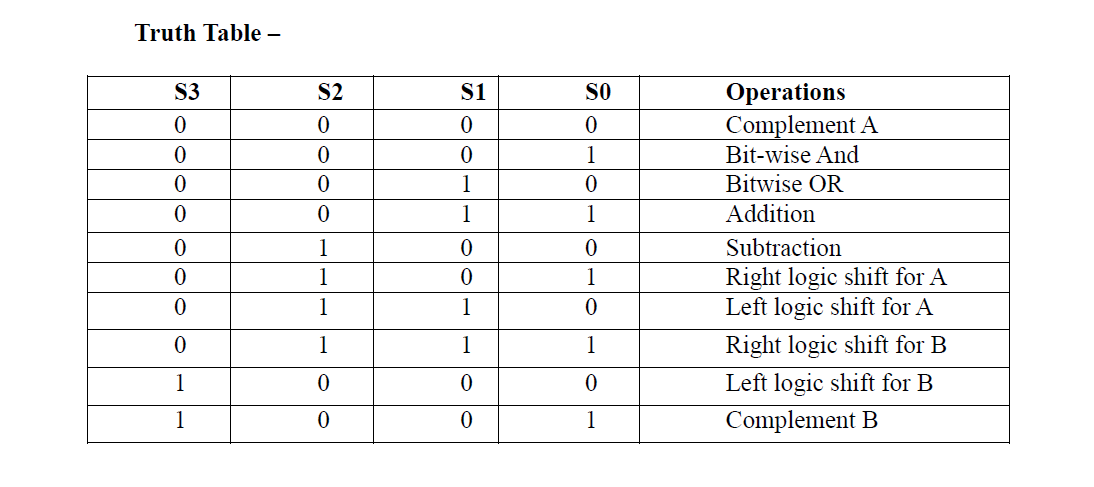
\includegraphics[scale=0.7]{Capture1}
\end{center}

\section{Procedure:}
For designing the 4 bit Arithmetic Logic Unit, I first designed a 4 bit Adder which will be used for 
Addition and subtraction. For complement, Bit shift and bitwise operations I used sequential behavioral model. \\
\begin{center}

Complement:\\
1' = 0\\
0' = 1\\ 
\vspace{3 mm}
Bitwise AND:\\
0 AND x = 0\\
1 AND 1 = 1\\ 
\vspace{3 mm}
Bitwise OR:\\
1 OR x = 1\\
0 OR 0 = 0\\
\vspace{3 mm}
XOR:\\
1 XOR 1 = 0\\
0 XOR 0 = 0\\
1 XOR 0 = 1\\
0 XOR 1 = 1\\

\end{center}

\section{Timing Diagrams}
\begin{figure}[!ht]
\centering
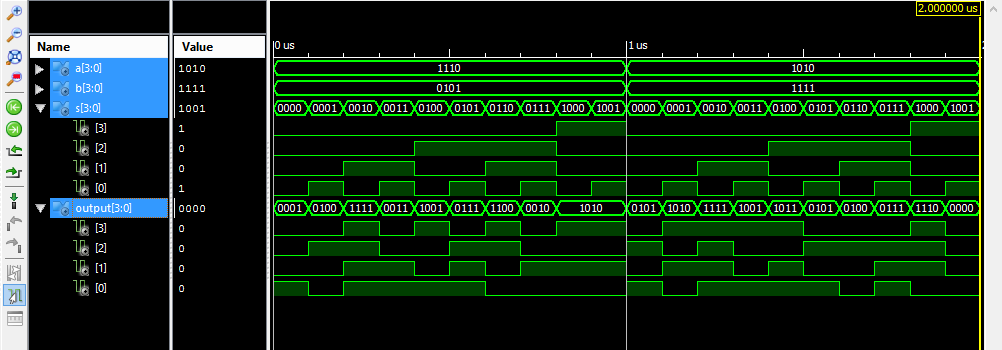
\includegraphics[width=1\textwidth]{Capture}
\caption{Timing Diagram for 4 bit Arithmetic Logic Unit}
\label{fig1}
\end{figure}

\section{Codes}
Here I have include working code for Arithmetic Logic Unit and 4-bit Adder.
\subsection{Arithmetic Logic Unit}
\begin{lstlisting}[style=vhdl]
-------------------------------------------------------------------------
-- Company: 
-- Engineer: 
-- 
-- Create Date:    14:20:01 03/04/2014 
-- Design Name: 
-- Module Name:    alu - Behavioral 
-- Project Name: 
-- Target Devices: 
-- Tool versions: 
-- Description: 
--
-- Dependencies: 
--
-- Revision: 
-- Revision 0.01 - File Created
-- Additional Comments: 
--
-------------------------------------------------------------------------
library IEEE;
use IEEE.STD_LOGIC_1164.ALL;

-- Uncomment the following library declaration if using
-- arithmetic functions with Signed or Unsigned values
--use IEEE.NUMERIC_STD.ALL;

-- Uncomment the following library declaration if instantiating
-- any Xilinx primitives in this code.
--library UNISIM;
--use UNISIM.VComponents.all;

entity alu is
    Port ( a : in  STD_LOGIC_VECTOR (3 downto 0);
           b : in  STD_LOGIC_VECTOR (3 downto 0);
           s : in  STD_LOGIC_VECTOR (3 downto 0);
           output : out  STD_LOGIC_VECTOR (3 downto 0));
end alu;

architecture Behavioral of alu is
signal c :std_logic_vector(3 downto 0);
signal c1 : std_logic_vector(3 downto 0);
signal c2 : std_logic_vector(3 downto 0);
signal temp : std_logic_vector(3 downto 0);

component add is
    Port ( a : in  STD_LOGIC_VECTOR (3 downto 0);
           b : in  STD_LOGIC_VECTOR (3 downto 0);
           output : out  STD_LOGIC_VECTOR (3 downto 0));
end component;

begin
c1(0) <= not b(0);
c1(1) <= not b(1);
c1(2) <= not b(2);
c1(3) <= not b(3);

add1: add 
	port map(a,b,c);	
add2: add 
	port map(c1,"0001",c2);
add3: add 
	port map(a,c2,temp);
process(a,b,s)
begin
case s is 
	when "0000" =>
		output(0) <= not a(0);
		output(1) <= not a(1);
		output(2) <= not a(2);
		output(3) <= not a(3);
	when "0001" =>
		output(0) <= a(0) and b(0);
		output(1) <= a(1) and b(1);
		output(2) <= a(2) and b(2);
		output(3) <= a(3) and b(3);
	when "0010" =>
		output(0) <= a(0) or b(0);
		output(1) <= a(1) or b(1);
		output(2) <= a(2) or b(2);
		output(3) <= a(3) or b(3);
	when "0011" =>
		output <= c;
	when "0100" =>
		output <= temp;
	when "0101" =>
		output(0) <= a(1);
		output(1) <= a(2);
		output(2) <= a(3);
		output(3) <= '0';
	when "0110" =>
		output(3) <= a(2);
		output(2) <= a(1);
		output(1) <= a(0);
		output(0) <= '0';
	when "0111" =>
		output(0) <= b(1);
		output(1) <= b(2);
		output(2) <= b(3);
		output(3) <= '0';
	when "1000" =>
		output(3) <= b(2);
		output(2) <= b(1);
		output(1) <= b(0);
		output(0) <= '0';
	when "1001" =>
		output(0) <= not b(0);
		output(1) <= not b(1);
		output(2) <= not b(2);
		output(3) <= not b(3);
	when others =>
		null;
end case;
end process;

end Behavioral;

\end{lstlisting}

\subsection{4 bit Adder}
\begin{lstlisting}[style=vhdl]
-------------------------------------------------------------------------
-- Company: 
-- Engineer: 
-- 
-- Create Date:    14:34:15 03/04/2014 
-- Design Name: 
-- Module Name:    add - Behavioral 
-- Project Name: 
-- Target Devices: 
-- Tool versions: 
-- Description: 
--
-- Dependencies: 
--
-- Revision: 
-- Revision 0.01 - File Created
-- Additional Comments: 
--
-------------------------------------------------------------------------
library IEEE;
use IEEE.STD_LOGIC_1164.ALL;

-- Uncomment the following library declaration if using
-- arithmetic functions with Signed or Unsigned values
--use IEEE.NUMERIC_STD.ALL;

-- Uncomment the following library declaration if instantiating
-- any Xilinx primitives in this code.
--library UNISIM;
--use UNISIM.VComponents.all;

entity add is
    Port ( a : in  STD_LOGIC_VECTOR (3 downto 0);
           b : in  STD_LOGIC_VECTOR (3 downto 0);
           output : out  STD_LOGIC_VECTOR (3 downto 0));
end add;


architecture Behavioral of add is
signal c1 :std_logic;
signal c2 : std_logic;
signal c3 : std_logic;
begin

output(0) <= a(0) xor b(0);
c1 <= a(0) and b(0);
output(1) <= a(1) xor b(1) xor c1;
c2 <= (a(1) and b(1)) or (a(1) and c1) or (b(1) and c1);
output(2) <= a(2) xor b(2) xor c2;
c3 <= (a(2) and b(2)) or (a(2) and c2) or (b(2) and c2);
output(3) <= a(3) xor b(3) xor c3;


end Behavioral;

\end{lstlisting}

\section{Inference}
In this assignment I inferred the following:\\
\verb|1.| Designing a basic Arithmetic Logic Unit\\
\verb|2.| Learned the Bit-wise operations  \\
\verb|3.| Learned the Bit Shifting \\
\verb|4.| Learned clock implementation \\
\end{document}
